\begin{figure}[h]
		\centering
		\frame{\includegraphics[width=1.0 \textwidth]{../Figures/Model_Overview.png}}
		\caption[Model overview for adaptive mode matching.]
		{\textbf{Model overview for adaptive mode matching.} 
		Using the LIGO digital system as a test bed for technology development has the advantage of easy integration at both LIGO sites.  The Syracuse system uses a Simulink style model with LIGO standard modules to read in data from the analog-to-digital converter (ADC) that contain signals from each RF photodiode segments, apply a phase rotation to get the signal into one quadrature (nominally I for a linear cavity) and normalize by the total power on the sensor.  Afterwards, the signals are sent to a master actuator function that diagonalizes the sensor signals into an actuators basis and sent to the digital-to-analog converter (DAC) to control the heater drivers.
		}
		\label{fig:AMM_overview}
\end{figure}

\begin{figure}[h]
	\centering
	\frame{\includegraphics[width=0.5 \textwidth]{../Figures/Oneil_ModeConverter.png}}
	\caption[Intensity profiles passing through a mode converter. ]
	{\textbf{Intensity profiles passing through a mode converter \cite{ONeilModeTransform}.} 
	The image in upper left corner represents the $m=3$ and $n=0$ Hermite Gauss (LG) mode which gets transformed through a converter for different rotations and phase advances.  The only combination which gives a symmetric Laguerre Gauss (LG) mode is $\phi=45\deg$ and $\theta=\pi/2$.  This gives some intuition about how to reverse this process to take an input LG mode and breaks the cylindrical symmetry so that the modal content can be sensed by a quadrant photodiode.
	}
	\label{fig:Oneil_modeconv}
\end{figure}

\begin{figure}[h]
	\centering
	\includegraphics[width=0.4 \textwidth]{../Figures/ModeConv_BPD_Pos.png}
	\includegraphics[width=0.4 \textwidth]{../Figures/ModeConv_BPD_Siz.png}
	\includegraphics[width=0.4 \textwidth]{../Figures/ModeConv_QPD_Pos.png}
	\includegraphics[width=0.4 \textwidth]{../Figures/ModeConv_QPD_Siz.png}
	\caption[Simulated error signals from MATLAB (QPD) and FINESSE (BPD).]
	{\textbf{Simulated error signals from MATLAB (QPD) and FINESSE (BPD).} 
	A numerical simulation of the error signal in reflection from a linear Fabry Perot cavity with different detectors when varying either the waist position ($\Delta z$) or Rayleigh range ($\Delta z_R$).  The error signal orthogonality at two different Gouy phases is demonstrated using both sensing schemes for active wavefront control.
	}
	\label{fig:ModeConv_err}
\end{figure}

\begin{figure}[h]
	\centering
	\includegraphics[width=1.0 \textwidth]{../Figures/ModeConv.png}
	\caption[Passing a bullseye mode through a $\pi/2$ mode converter.]
	{\textbf{Passing a bullseye mode through a $\pi/2$ mode converter.} The reflected fields of a well aligned Fabry-Perot cavity with a slight mode mismatch will have a large contribution from the $\ket{\text{HG}_{20}} + \ket{\text{HG}_{02}}$ mode which is cylindrically symmetric.  After passing through a cylindrical telescope which has a $\pi/2$ phase advance for one axis, there is a relative sign flip which breaks the the symmetry and the error signal can be extracted with an RF quadrant photodiode.
	}
	\label{fig:ModeConv}
\end{figure}